\documentclass[10pt]{article}
\usepackage[a4paper,margin=1.65cm]{geometry}
\usepackage[T1]{fontenc}
\usepackage[english,french]{babel}
\frenchsetup{SmallCapsFigTabCaptions=false}
\addto\captionsfrench{\renewcommand{\tablename}{Tableau}}
\usepackage{lmodern}
\usepackage{microtype}
\usepackage{graphicx}
\usepackage{booktabs}
\usepackage{tabularx}
\usepackage{array}
\usepackage{amsmath}
\usepackage{xcolor}
\usepackage[hidelinks]{hyperref}
\usepackage{caption}
\captionsetup{font=small,labelfont=bf}
\setlength{\parskip}{3.5pt}
\graphicspath{{../research/timecourse/figures/}{../research/person/figures/}{../research/revision/figures/}}
\newcolumntype{L}[1]{>{\raggedright\arraybackslash}p{#1}}
\newcolumntype{Y}{>{\raggedright\arraybackslash}X}

\title{Ce que le cerveau et le corps montrent pendant un stress aigu chez 314 personnes}
\author{Équipe 12 : Mathias Chebbah, Aurélien Saint-Grégoire, Ashley Russo\\
\small HABS Neuro-AI Hackathon, Université Paris-Saclay, novembre 2026}
\date{}

\begin{document}
\maketitle

\begin{abstract}
\noindent Nous avons mesuré comment le cerveau et le corps réagissent à un stress aigu bref chez 314 volontaires sains (22\,974 essais, 252 vidéos de 10~s, jeu de données HABS). Nous avons aussi testé ce que les détecteurs multimodaux arrivent vraiment à lire. Six résultats ressortent.

Premièrement, le critère de stress (valence au plus 4 et arousal au moins 6) contient 89,2\,\% d'émotions négatives en premier choix (97,2\,\% sur les trois choix) et 5,3\,\% d'états incohérents. Durcir le seuil jusqu'à valence au plus 2 et arousal au moins 8 porte la pureté à 95,3\,\% et double les réponses de la conductance cutanée ($d$ passe de $+0{,}14$ à $+0{,}34$) et du delta EEG ($+0{,}13$ à $+0{,}30$). Ce durcissement réduit en même temps de moitié le ralentissement cardiaque ($-0{,}11$ à $-0{,}04$). Le seuil valence au plus 3 et arousal au moins 7 maximise la détection (AUC 0,549). Deuxièmement, les émotions négatives ne partagent pas un profil unique. La peur cumule ralentissement cardiaque ($-0{,}20$), conductance cutanée ($+0{,}25$), respiration superficielle ($-0{,}11$) et baisse d'alpha ($-0{,}12$). Le dégoût ralentit le cœur ($-0{,}20$) et élève le delta ($+0{,}15$) sans faire monter la conductance cutanée. La tristesse reste plate sur tous les capteurs. Le clustering sans étiquette ne retrouve ni le stress ni les émotions ($\mathrm{ARI} < 0{,}009$). Troisièmement, l'intervalle cardiaque RR s'allonge ($+5{,}1$~ms, $d = +0{,}116$), mais l'intervalle PR et le segment PR restent nuls ($-0{,}05$~ms, $d = -0{,}002$). La baisse apparente du QTc de Bazett ($-0{,}092$) disparaît après contrôle sur $\Delta\mathrm{RR}$ ($-0{,}007$). La réponse cardiaque sur 10~s relève donc d'un freinage vagal sinusal sans accélération adrénergique mesurable du nœud atrio-ventriculaire. En EEG, la volatilité temporelle précoce augmente fortement (saut maximal de 1~s en delta, $d = +0{,}151$) et l'organisation spatiale s'homogénéise au début puis se focalise après la vidéo (entropie spatiale alpha, $d = -0{,}076$). Quatrièmement, le potentiel évoqué cardiaque (HEP) ne varie pas sous stress sur l'EEG prétraité par ICA ($d = +0{,}039$) ni sur l'EEG brut sans ICA ($d = +0{,}038$). Cinquièmement, opposer les spectateurs stressés aux spectateurs vraiment calmes devant la même vidéo fait passer l'AUC à vidéo fixe de 0,525 à 0,564. Les spectateurs calmes devant une vidéo consensuellement stressante ne montrent ni ralentissement cardiaque ($-0{,}49$~bpm) ni hausse de conductance cutanée ($+0{,}014\,\mu$S). Seule la baisse d'alpha reste automatique ($d = -0{,}33$ à $-0{,}41$). La sensibilité individuelle suit le bêta et le gamma frontaux ($-0{,}035$ et $-0{,}039$) ainsi que le delta centro-pariétal, qui résiste à 93\,\% à un contrôle oculaire pré-ICA. Sixièmement, remplacer les tranches de 1~s par 4 phases physiologiques enrichies fait monter l'AUC sur personnes et thèmes inédits de 0,526 à 0,589 (modèle linéaire) et 0,586 (régression Ridge continue sur valence et arousal, meilleur modèle global avec 0,576 en développement et 0,656 contre les essais relaxés). Les ondes PR et les classifieurs non linéaires (GBDT et MLP) n'améliorent pas la généralisation sur de nouveaux thèmes.
\end{abstract}

\section{Pourquoi nous avons mené cette étude}

Deux questions pratiques guident ce travail. D'abord, que font exactement le cerveau et le corps pendant une réaction de stress aigu brève, dans quel ordre, sur quelles zones du scalp et sous quelle branche du système nerveux autonome ? Ensuite, qu'est-ce qu'un détecteur multimodal lit vraiment chez une personne nouvelle face à une situation nouvelle ?

Ces deux questions dépassent tout contexte professionnel particulier. Elles intéressent le neurofeedback, les études de neurosciences affectives et le monitorage clinique des patients qui ne peuvent pas parler. Un nouveau-né ou un jeune enfant qui ressent une douleur aiguë, un patient en \emph{locked-in syndrome}, un patient dans le coma ou un patient sous anesthésie générale ne peuvent pas donner de note verbale. Un biomarqueur utile dans ces situations doit séparer une souffrance vécue d'un simple réflexe sensoriel déclenché par un stimulus fort.

Le jeu de données HABS réunit 314 adultes sains qui ont regardé 252 clips audiovisuels de 10~s, soit 22\,974 essais valides enregistrés avec EEG 64 voies, ECG, conductance cutanée et respiration. HABS ne contient ni tâche cognitive, ni cortisol, ni douleur physique. Sa force est sa taille (314 participants contre 15 à 50 dans la plupart des études de laboratoire \cite{palomba2000,hagenaars2014,schubring2019}) et sa structure croisée. Chaque vidéo a été vue par 13 à 234 personnes différentes (médiane 83). Cette structure permet de comparer des personnes différentes devant exactement le même stimulus, et d'éviter le biais déjà décrit où un classifieur EEG reconnaît simplement la vidéo plutôt que l'émotion \cite{giannakakis2015,gerster2026}.

Ce travail répond à six critiques méthodologiques adressées à nos analyses antérieures (études 04 à 06) :
\begin{enumerate}
\item vérifier que le critère valence et arousal capture bien des états de stress, puis mesurer l'effet d'un durcissement du seuil ;
\item entraîner des modèles directement sur les émotions déclarées en premier choix et tester une approche non supervisée ;
\item remplacer le découpage figé à 1~s par 4 phases physiologiques, mesurer les ondes ECG P-QRS-T (notamment le segment PR lié au nœud atrio-ventriculaire), ajouter la volatilité temporelle et l'homogénéité spatiale EEG, et tester des architectures séquentielles ;
\item vérifier sur l'EEG brut non traité (\texttt{CURATED}) que le prétraitement ICA n'a pas effacé un signal cerveau-cœur ;
\item corriger l'analyse à vidéo fixe en éliminant la dilution par les essais intermédiaires et tester si la réponse physiologique est graduée ou en tout-ou-rien ;
\item cartographier les régions EEG liées à la sensibilité individuelle au stress et contrôler l'effet des clignements sur le delta.
\end{enumerate}

Nous avons figé ce protocole dans \texttt{journal/07\_comprehensive\_revision.md} avant de lancer les nouveaux calculs.

\section{Comment nous avons préparé et analysé les données}

\subsection{Données, capteurs et prétraitement}

Nous analysons les 22\,974 essais de HABS dont les marqueurs temporels concordent entre métadonnées et fichiers BDF à moins de 25~ms (314 participants, 5 cohortes, 508 enregistrements, 252 vidéos regroupées en 84 thèmes). Dans la table distribuée \texttt{labels\_train.csv}, la colonne \texttt{flagged\_outliers} vaut 0 sur tous les 22\,974 essais retenus. Les cohortes 2 à 5 ($n = 17\,142$, 209 personnes) contiennent des notes continues de valence et d'arousal entre 1 et 9, plus 1 à 3 émotions choisies par le spectateur parmi 12 catégories (\texttt{self\_reported\_emotion\_1} à \texttt{3}). La cohorte 1 ($n = 5\,832$, 105 personnes) contient des notes entières sans sélection d'émotion.

Les quatre capteurs sont enregistrés à 1\,000~Hz (ANT Neuro eego 64 et SenseBox). L'EEG comprend 64 électrodes en montage 10--10. L'ECG utilise une seule dérivation bipolaire sous-claviculaire (équivalent D1), ce qui exclut toute comparaison spatiale entre plusieurs dérivations ECG. La conductance cutanée est mesurée sur la main non dominante et convertie en $\mu$S par la courbe constructeur. Une ceinture thoracique basse mesure la respiration. L'oculométrie est exclue sur consigne des organisateurs pour défaut de synchronisation.

Le dossier \texttt{PREPROCESSED} fourni par HABS retire les électrodes T9 et T10, applique un filtre coupe-bande à 50~Hz sur les capteurs périphériques, filtre l'EEG entre 0,5 et 48~Hz, le re-référence à la moyenne des 62 électrodes restantes (CAR), puis applique une ICA Picard avec \emph{ICLabel}. Les composantes dépassant 0,75 pour les artefacts oculaires ou 0,90 pour le muscle, le secteur ou un canal défectueux sont retirées. La classe cardiaque d'ICLabel ne figure pas dans ces seuils, mais une activité covariante avec le cœur peut quand même passer dans une autre composante rejetée. Nous testons donc directement le dossier brut \texttt{CURATED} sans ICA.

\subsection{Audit du critère, émotions brutes et clustering non supervisé}

Le label \texttt{final\_emotion\_label} de HABS utilise déjà la valence et l'arousal. L'employer pour valider notre règle de stress serait circulaire. Nous auditons donc le critère uniquement sur le premier choix brut du spectateur (\texttt{self\_reported\_emotion\_1}, complété par les rangs 2 et 3 dans \texttt{criterion\_full}), disponible sur 100\,\% des cohortes 2 à 5. Nous classons les 12 émotions en quatre groupes : menace aiguë (colère, peur, dégoût), négatif non menaçant (tristesse, culpabilité), surprise, et émotions incohérentes avec le stress (joie, excitation, relaxation, sensualité, neutre, curiosité). Nous balayons dix seuils de valence et d'arousal, du quadrant ouvert ($V < 5$ et $A > 5$) jusqu'au coin extrême ($V \le 2$ et $A \ge 8$).

Pour tester les émotions directement, nous entraînons neuf classifieurs binaires et un classifieur à 5 classes (peur, colère, dégoût, tristesse, autre) en validation croisée $3 \times 3$ par personnes et par thèmes. Un piège technique est apparu en développement. Comme les thèmes vidéo regroupent certaines émotions, les trois plis de thèmes n'ont pas la même fréquence d'entraînement pour une émotion donnée. Sans équilibrage, l'intercept de la régression logistique change d'un pli à l'autre et produit des AUC artificiellement sous 0,50 quand on réunit les prédictions (0,387 pour la colère). L'option \texttt{class\_weight="balanced"} fixe la probabilité a priori d'entraînement à 0,50 dans chaque pli et supprime ce biais sans fuite de données. Pour les réseaux de neurones, nous appliquons l'ajustement bayésien exact du rapport de vraisemblance $\log\frac{p}{1-p} - \log\frac{\pi_{\text{train}}}{1-\pi_{\text{train}}}$.

Pour l'analyse non supervisée, nous centrons 36 variables physiologiques par participant (fréquence cardiaque, conductance cutanée, amplitude et rythme respiratoires en phases précoce et tardive, et 6 régions fois 5 bandes EEG). Sans exposer aucune étiquette, nous appliquons une ACP puis $k$-means ($k = 2$ à 6) et des mélanges gaussiens ($k = 2$ à 5) sur les 8 premières composantes. Nous mesurons l'accord avec le stress, les émotions, le thème et la vidéo par l'indice de Rand ajusté (ARI) et l'information mutuelle normalisée (NMI).

\subsection{Extraction en 4 phases, délinéation ECG P-QRS-T et descripteurs EEG}

Le script \texttt{decoding/\allowbreak rich\_extract.py} (exécuté sur le backend HABS, job \texttt{20261123T004720-2ea585}) calcule 650 variables par essai sur quatre fenêtres physiologiques : référence ($-3$ à $0$~s), précoce ($0$ à $5$~s), tardif ($5$ à $10$~s) et post-exposition ($10$ à $12$~s), plus la fenêtre complète ($0$ à $10$~s) pour l'ECG. Ces quatre fenêtres complètent l'extraction seconde par seconde de l'étude 05.

L'inspection des tracés ECG bruts a révélé que la dérivation sous-claviculaire est inversée dans 96,6\,\% des essais (ondes P et T négatives, onde S positive). La correction automatique de NeuroKit2 échoue sur ces tracés et ne retrouvait que 2\,\% des ondes T sur l'échantillon test. Nous avons donc écrit \texttt{delineate\_ecg} dans \texttt{decoding/\allowbreak rich\_extract.py}. L'algorithme détecte les complexes QRS (5 à 25~Hz), construit le battement médian par enregistrement, choisit la polarité par vote conjoint des ondes P ($-240$ à $-70$~ms) et T ($+130$ à $+420$~ms), rejette les battements dont la corrélation QRS au gabarit tombe sous 0,70 (99,2\,\% de battements conservés en médiane), puis repère sur chaque battement $\mathrm{P}_{\text{on}}$, $\mathrm{P}_{\text{pic}}$, $\mathrm{P}_{\text{off}}$, $\mathrm{QRS}_{\text{on}}$, R, $\mathrm{QRS}_{\text{off}}$, $\mathrm{T}_{\text{pic}}$ et $\mathrm{T}_{\text{off}}$. Nous calculons pour chaque phase la fréquence cardiaque, RR, RMSSD, le pic PR ($\mathrm{R} - \mathrm{P}_{\text{pic}}$), l'intervalle PR clinique ($\mathrm{QRS}_{\text{on}} - \mathrm{P}_{\text{on}}$), le segment PR pur ($\mathrm{QRS}_{\text{on}} - \mathrm{P}_{\text{off}}$), QRS, QT, QTc de Bazett ($\mathrm{QT}/\sqrt{\mathrm{RR}}$), QTc de Fridericia ($\mathrm{QT}/\mathrm{RR}^{1/3}$), le pic RT et le ratio T sur R. Chaque mesure morphologique est aussi testée dans une régression intra-personne ajustée sur $\Delta\mathrm{RR}$ pour séparer un effet intrinsèque d'un couplage à la fréquence cardiaque.

Pour l'EEG, nous calculons par densité spectrale de Welch dans chaque phase et chaque bande ($\delta, \theta, \alpha, \beta, \gamma$) quatre groupes de mesures :
\begin{enumerate}
\item la log-puissance moyenne dans 6 régions du scalp (frontal, central, temporal gauche, temporal droit, pariétal, occipital) ;
\item quatre indices d'homogénéité spatiale sur les 62 électrodes : écart-type inter-canaux (\texttt{sp\_std}), écart interquartile (\texttt{sp\_iqr}), entropie de Shannon normalisée (\texttt{sp\_ent} entre 0 et 1, où 1 indique une puissance uniforme sur tout le scalp) et écart-type entre régions ;
\item trois gradients et asymétries : gradient antéro-postérieur (frontal moins occipital), asymétrie frontale droite moins gauche (FAA) et asymétrie temporale ;
\item trois indices de volatilité temporelle sur les sous-fenêtres de 1~s : écart-type temporel (\texttt{tvar}), pente linéaire (\texttt{tslope}) et plus grand saut entre deux secondes consécutives (\texttt{maxjump}).
\end{enumerate}

Pour fournir la structure temporelle aux modèles, nous ajoutons les transitions explicites de phase $\Delta(t\to t+1)$ (0 en référence, précoce moins référence, tardif moins précoce, post moins tardif). Nous extrayons enfin l'amplitude crête-à-crête sur Fp1 et Fp2 entre 0 et 2~s sur l'EEG brut \texttt{CURATED} comme contrôle direct des clignements pré-ICA.

\subsection{Contrôle du potentiel évoqué cardiaque sans ICA}

Pour vérifier si l'ICA retire un signal cortical lié au battement cardiaque, nous extrayons le potentiel évoqué cardiaque (HEP) directement depuis les fichiers bruts \texttt{CURATED} sans ICA. Nous appliquons exactement les mêmes étapes que sur \texttt{PREPROCESSED} : exclusion de T9 et T10, moyenne commune des 62 électrodes, filtre 0,5 à 30~Hz, découpage de $-200$ à $+600$~ms en 16 tranches de 50~ms autour des mêmes pics R, correction par la ligne de base ($-200$ à $-50$~ms), et rejet des époques dépassant 100\,$\mu$V (ainsi qu'un seuil élargi à 200\,$\mu$V). En soustrayant \texttt{PREPROCESSED} à \texttt{CURATED} essai par essai, nous obtenons le signal exact retiré par l'ICA. Le test principal porte sur la fenêtre 250 à 600~ms en frontal et central, avant et après ajustement sur l'amplitude ECG et sur RR \cite{parkblanke2019}.

\subsection{Part partagée, contraste à vidéo fixe et sensibilité individuelle}

Pour éviter les étiquettes ambiguës de « personne » et « situation », nous définissons deux grandeurs précises pour chaque essai d'un spectateur $p$ devant une vidéo $v$. La part partagée est la moyenne des notes centrées des autres spectateurs de la même vidéo $v$ (au moins 9 autres personnes, sans inclure $p$). Elle regroupe l'effet sensoriel du stimulus et la réaction humaine consensuelle. La part propre est l'écart entre la note du spectateur $p$ et cette moyenne partagée. Elle mesure sa sensibilité personnelle à ce clip.

Devant une vidéo consensuellement stressante, opposer les spectateurs stressés à « tous les autres » mélange des spectateurs vraiment calmes et des spectateurs presque au seuil de stress. Nous auditons donc la distribution du taux de stress sur les 252 vidéos, puis nous testons à vidéo fixe trois contrastes propres : les vidéos polarisantes (taux de stress entre 20 et 80\,\%), le contraste non adjacent entre spectateurs stressés ($V \le 4, A \ge 6$) et spectateurs calmes ($V \ge 5, A \le 5$, puis version stricte $V \ge 5{,}5, A \le 4{,}5$), et les contrastes isolant un seul axe à la fois (valence pure et arousal pur). Nous construisons ensuite une matrice $2 \times 2$ croisant trois niveaux de consensus vidéo (bas au plus 10\,\%, polarisant de 20 à 55\,\%, haut au moins 50\,\%) et trois états vécus (très calme, intermédiaire, stressé). Nous mesurons enfin les courbes dose-réponse sur 8 tranches de valence et d'arousal.

Au niveau individuel ($N = 314$), nous mesurons la sensibilité-trait de chaque personne par son écart moyen de taux de stress par rapport aux autres spectateurs des mêmes vidéos, ajusté sur la cohorte. Nous relions cet indice à sa fréquence cardiaque de repos et à son EEG pré-stimulus ($-3$ à $0$~s).

\subsection{Benchmark des 12 modèles et inférence}

Les 12 configurations de détection sont testées dans \texttt{decoding/revision.py} sur un nouveau découpage déterministe personnes par thèmes (\texttt{habs-revision-2026-11-23}). Le jeu de développement compte 12\,052 essais (249 personnes, 60 thèmes) évalués en validation croisée $3 \times 3$. Trois tests scellés ouverts une seule fois mesurent la généralisation sur personnes et thèmes nouveaux (1\,646 essais, 65 personnes, 24 thèmes), personnes nouvelles (3\,285 essais) et thèmes nouveaux (5\,991 essais). Nous comparons les tranches de 1~s, les 4 phases, chaque bloc de nouvelles variables, la régression Ridge continue sur valence et arousal, le \emph{HistGradientBoosting} (GBDT), une banque de 48 filtres convolutifs 1D multi-échelles sur la série de 12~s (avec dérivées première et seconde), et un MLP calibré. Tous les intervalles de confiance à 95\,\% utilisent 2\,000 tirages bootstrap sur les personnes, ou sur les vidéos pour les tests à vidéo fixe \cite{varoquaux2018}.

\section{Résultats}

\subsection{Le critère de stress est valide, mais durcir le seuil dissocie la peau et le cœur}

Sur les 3\,938 essais inclus dans le critère standard ($V \le 4$ et $A \ge 6$) dans les cohortes 2 à 5, 89,2\,\% des participants choisissent une émotion négative en premier rang (figure~\ref{fig:criterion}A). Quatre émotions dominent : colère (25,7\,\%), peur (23,9\,\%), dégoût (22,9\,\%) et tristesse (14,9\,\%). Viennent ensuite la surprise (5,5\,\%), la curiosité (2,7\,\%), la culpabilité (1,8\,\%), neutre (1,4\,\%) et l'excitation (1,1\,\%). La relaxation (0,13\,\%), la sensualité (0,03\,\%) et la joie (0,03\,\%) sont quasi absentes. Sur l'ensemble des trois choix déclarés, 97,2\,\% des essais incluent une émotion négative et 90,1\,\% une menace aiguë (colère, peur ou dégoût). Parmi les 5,3\,\% d'essais ($n = 209$) ayant un premier choix incohérent, 69,9\,\% citent une émotion négative en deuxième ou troisième choix.

\begin{figure}[t]
\centering
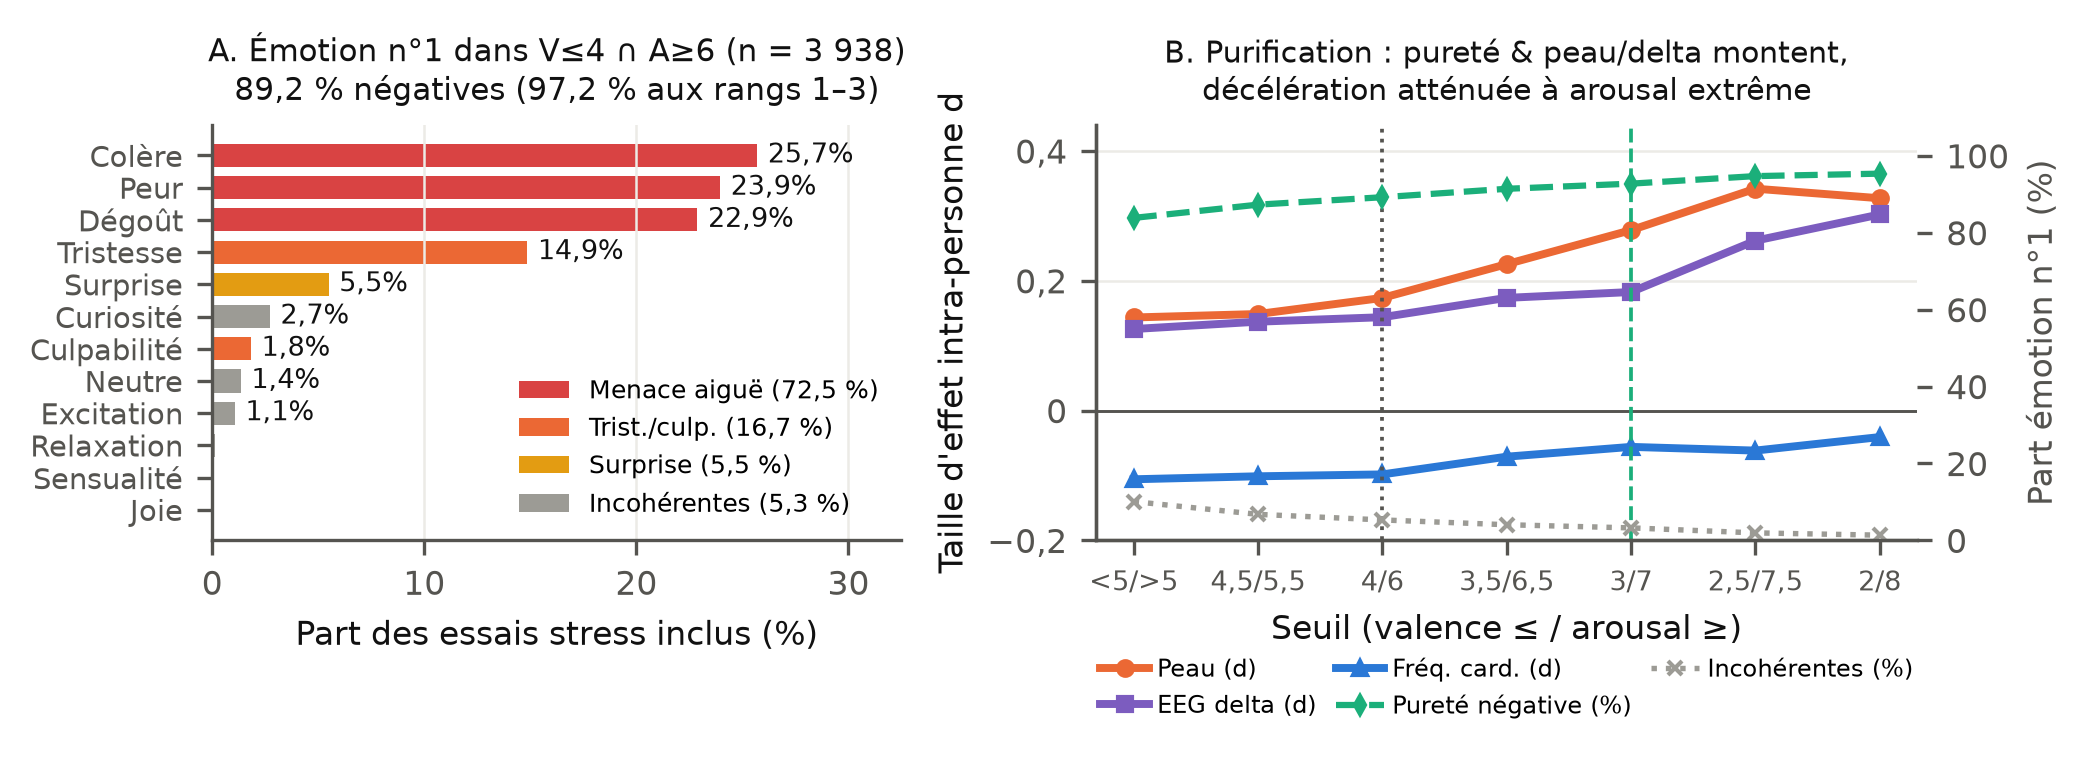
\includegraphics[width=\linewidth]{fig1_criterion_fr.png}
\caption{\textbf{Audit et purification du critère de stress.} \textbf{A.} Émotion déclarée en premier choix dans le critère $V \le 4$ et $A \ge 6$ (cohortes 2 à 5, $n = 3\,938$). \textbf{B.} Effet du durcissement du seuil sur la pureté et sur les tailles d'effet physiologiques intra-personne.}
\label{fig:criterion}
\end{figure}

Le balayage des seuils met au jour deux faits utiles (figure~\ref{fig:criterion}B et tableau~\ref{tab:purification}). D'abord, le quadrant ouvert ($V < 5$ et $A > 5$) admet 10,1\,\% d'émotions incohérentes. Passer à $V \le 4$ et $A \ge 6$ divise ce taux par deux (5,3\,\%). Le seuil $V \le 3$ et $A \ge 7$ (13,4\,\% des essais, 241 personnes) porte la pureté négative à 92,7\,\% et maximise la détection (AUC intra-personne 0,549 [0,535 ; 0,563], AUC à vidéo fixe 0,527 [0,510 ; 0,543]). Au-delà ($V \le 2$ et $A \ge 8$, 137 personnes), la pureté atteint 95,3\,\% mais la baisse d'effectif réduit la détection (AUC 0,540).

Ensuite, durcir le seuil fait diverger les deux branches autonomes. Entre $V < 5, A > 5$ et $V \le 2{,}5, A \ge 7{,}5$, l'effet sur la conductance cutanée passe de $+0{,}143$ à $+0{,}342$ et l'effet sur le delta EEG double ($+0{,}126$ à $+0{,}302$ à $2$ et $8$). À l'inverse, le ralentissement cardiaque baisse de moitié ($-0{,}106$ à $-0{,}041$). Les seuils asymétriques confirment le rôle de l'arousal. À valence fixée ($V \le 4$), relever l'arousal de $>5$ à $\ge 7$ fait passer la conductance cutanée de $+0{,}148$ à $+0{,}286$ et réduit le ralentissement cardiaque de $-0{,}099$ à $-0{,}052$. Aux très hauts niveaux d'activation, la poussée sympathique cardiaque s'oppose au freinage vagal.

\begin{table}[t]
\centering\small
\begin{tabular}{@{}lrrrrrrr@{}}
\toprule
Seuil ($V$ et $A$) & Essais (\%) & Pureté nég. & Menace & Incoh. & Peau ($d$) & Cœur ($d$) & AUC intra (pers.)\\
\midrule
$V < 5$ et $A > 5$ & 6\,661 (29,0\,\%) & 83,8\,\% & 66,6\,\% & 10,1\,\% & $+0{,}143$ & $-0{,}106$ & 0,537 (292)\\
$V \le 4$ et $A \ge 6$ (réf.) & 5\,510 (24,0\,\%) & 89,2\,\% & 72,5\,\% & 5,3\,\% & $+0{,}173$ & $-0{,}098$ & 0,540 (287)\\
$V \le 3$ et $A \ge 7$ (opt.) & 3\,081 (13,4\,\%) & 92,7\,\% & 78,7\,\% & 3,2\,\% & $+0{,}278$ & $-0{,}056$ & \textbf{0,549} (241)\\
$V \le 2{,}5$ et $A \ge 7{,}5$ & 1\,874 (8,2\,\%) & 94,7\,\% & 81,4\,\% & 1,9\,\% & $\mathbf{+0{,}342}$ & $-0{,}062$ & 0,526 (173)\\
$V \le 2$ et $A \ge 8$ & 1\,351 (5,9\,\%) & \textbf{95,3\,\%} & \textbf{84,7\,\%} & \textbf{1,4\,\%} & $+0{,}327$ & $-0{,}041$ & 0,540 (137)\\
\bottomrule
\end{tabular}
\caption{Pureté sur le premier choix brut, effets physiologiques intra-personne et AUC logistique équilibrée selon le seuil de stress.}
\label{tab:purification}
\end{table}

\subsection{Les émotions négatives diffèrent entre elles et le non-supervisé échoue}

L'analyse par émotion déclarée en premier choix ($n = 17\,142$, $N = 209$) montre que le quadrant stress mélange des profils physiologiques distincts (figure~\ref{fig:emotions}A), en accord avec la méta-analyse de Siegel et al.\ \cite{siegel2018}.
\begin{itemize}
\item La peur ($n = 1\,425$) active tous les capteurs : ralentissement cardiaque ($d = -0{,}20$ [$-0{,}28 ; -0{,}11$]), hausse de conductance cutanée ($+0{,}25$ [$+0{,}13 ; +0{,}36$]), respiration plus superficielle ($-0{,}11$) et baisse d'alpha ($-0{,}12$).
\item Le dégoût ($n = 1\,816$) ralentit autant le cœur ($-0{,}20$ [$-0{,}28 ; -0{,}12$]) et élève le delta ($+0{,}15$), mais laisse la conductance cutanée ($+0{,}06$) et l'alpha ($-0{,}01$) inchangés \cite{palomba2000}.
\item La colère ($n = 1\,453$) élève le delta ($+0{,}16$) avec des variations faibles sur la conductance cutanée ($+0{,}09$) et le cœur ($-0{,}08$).
\item La tristesse ($n = 1\,470$) ne déplace aucun capteur (cœur $-0{,}04$, conductance cutanée $0{,}00$, respiration $+0{,}04$, alpha $+0{,}08$). Sa présence dans le critère (14,9\,\%) dilue donc le signal de menace aiguë.
\item La joie accélère le cœur ($+0{,}09$ [$+0{,}01 ; +0{,}17$]). La relaxation approfondit la respiration ($+0{,}23$) et augmente l'alpha ($+0{,}12$).
\end{itemize}

\begin{figure}[t]
\centering
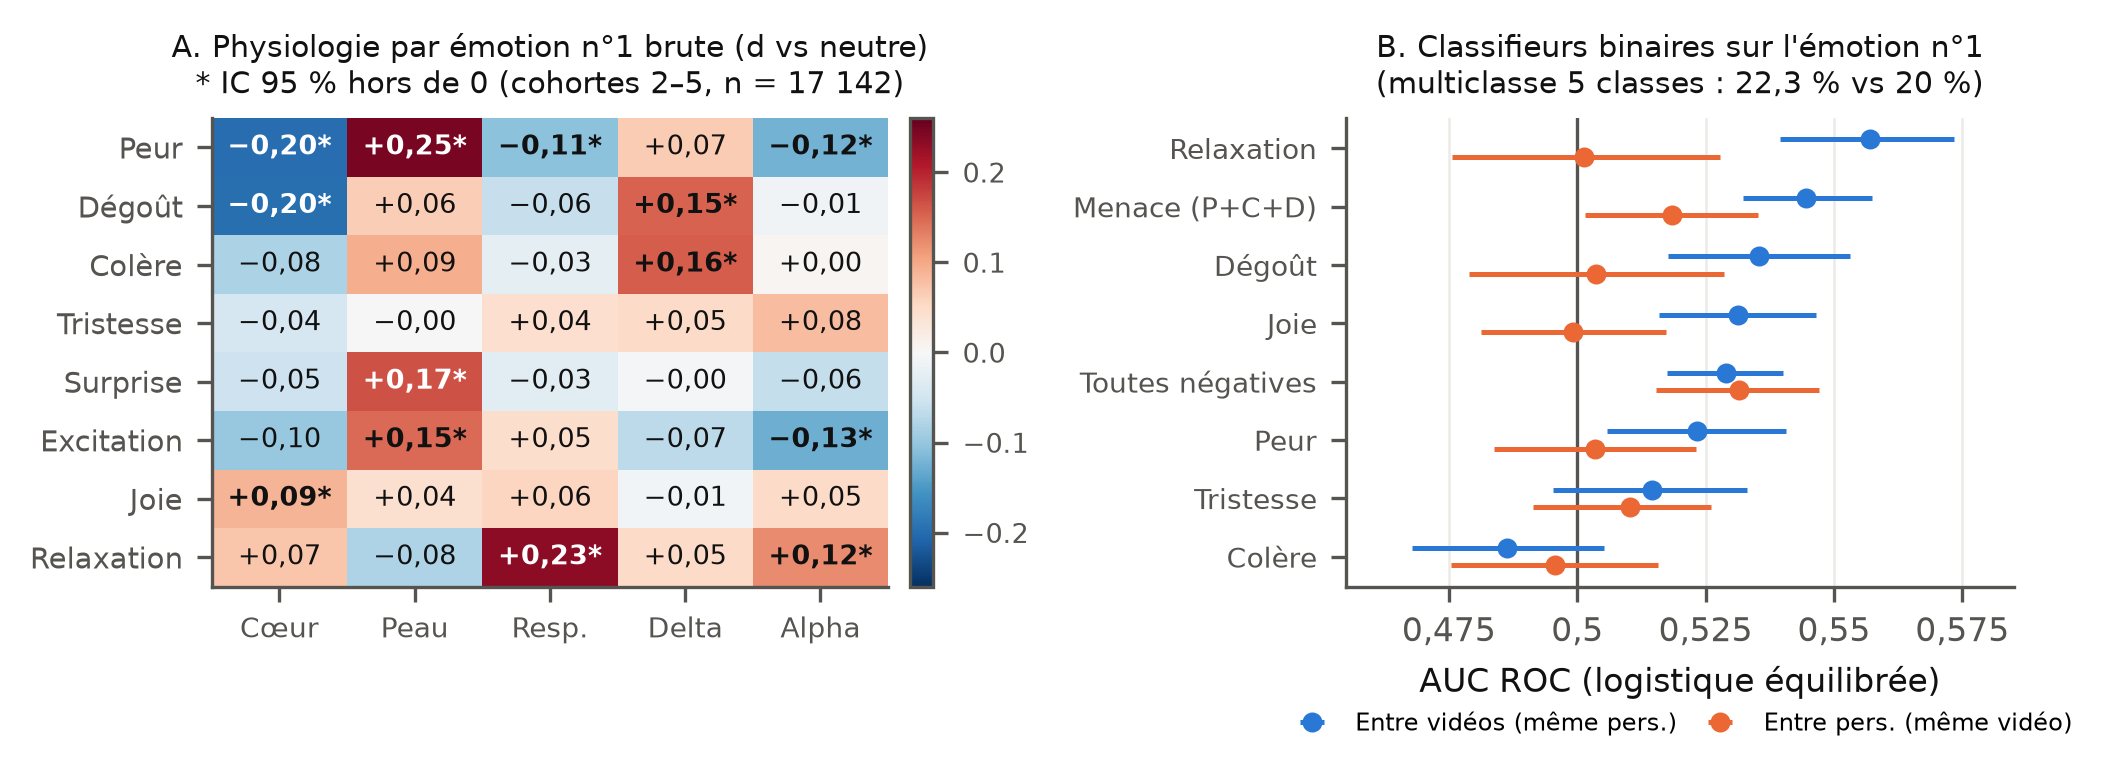
\includegraphics[width=\linewidth]{fig2_emotions_fr.png}
\caption{\textbf{Signatures physiologiques et classification directe sur l'émotion déclarée en premier choix.} \textbf{A.} Taille d'effet intra-personne contre neutre dans les cohortes 2 à 5. \textbf{B.} AUC des classifieurs binaires équilibrés entre vidéos d'une même personne (bleu) et entre spectateurs d'une même vidéo (orange).}
\label{fig:emotions}
\end{figure}

Les classifieurs binaires entraînés sur chaque émotion confirment qu'aucun sous-groupe n'est fortement séparable sur de nouveaux thèmes (figure~\ref{fig:emotions}B). Les AUC intra-personne valent 0,557 [0,540 ; 0,573] pour la relaxation, 0,545 [0,532 ; 0,558] pour la menace aiguë (0,550 contre neutre), 0,536 pour le dégoût, 0,531 pour la joie, 0,529 pour toutes négatives, 0,523 pour la peur, 0,515 pour la tristesse et 0,486 pour la colère. Pour la classe toutes négatives, l'AUC à vidéo fixe atteint 0,532 [0,515 ; 0,547] avec un effet propre non nul de la fréquence cardiaque ($\beta_{\text{propre}} = -0{,}032$ [$-0{,}049 ; -0{,}014$]). Le classifieur unifié à 5 classes obtient 22,3\,\% d'exactitude équilibrée contre 20,0\,\% au hasard.

Sans étiquette, l'ACP sur les 36 variables centrées par personne capte surtout l'état EEG global. PC1 (44,4\,\% de la variance) reflète la puissance large bande thêta et bêta, PC2 (10,2\,\%) le gamma, et PC3 (8,3\,\%) l'alpha pariéto-occipital (corrélé à l'arousal à $r = -0{,}060$). PC4 capte un axe cardio-respiratoire faiblement lié au stress ($r = -0{,}054$). Les clusters $k$-means ($k = 2$ à 6) et GMM ($k = 2$ à 5) ne retrouvent ni le stress ($\mathrm{ARI} \in [-0{,}006 ; +0{,}008]$, $\mathrm{NMI} \le 0{,}0006$, taux de stress entre 23,1 et 26,6\,\% dans les 4 clusters) ni les 5 émotions ($\mathrm{NMI} \le 0{,}0015$). Leur lien avec l'identité de la vidéo est dix fois plus grand ($\mathrm{NMI} = 0{,}009$ à 0,013).

\subsection{Le cœur ralentit sans raccourcir PR et la volatilité EEG augmente tôt}

En résolution 1~s (figure~\ref{fig:curves}), les quatre systèmes bougent dans un ordre fixe. Le delta EEG monte avant 1~s ($d = +0{,}11$ à $+0{,}14$). La fréquence cardiaque baisse dès 1~s (jusqu'à $-0{,}12$ à 7~s). La respiration devient moins ample de 2 à 6~s. La conductance cutanée monte à partir de 4~s, avec exactement le même délai sur 52 sujets tenus à l'écart ($d$ jusqu'à $+0{,}25$) \cite{bradley2009,benedek2010}. La fréquence cardiaque et la respiration suivent surtout la valence négative (contre excitation à arousal égal, cœur $-0{,}075$ et respiration $-0{,}078$). La conductance cutanée suit l'arousal (contre négatif calme $+0{,}13$, contre excitation nul) \cite{lang1993}. Sur 10~s, la fréquence cardiaque concorde avec la fenêtre de 60~s ($r = 0{,}94$, limites $\pm 7{,}3$~bpm), mais la RMSSD est trop bruyante ($r = 0{,}43$ intra-enregistrement et $0{,}22$ entre deux phases de 5~s) \cite{munoz2015}.

\begin{figure}[t]
\centering
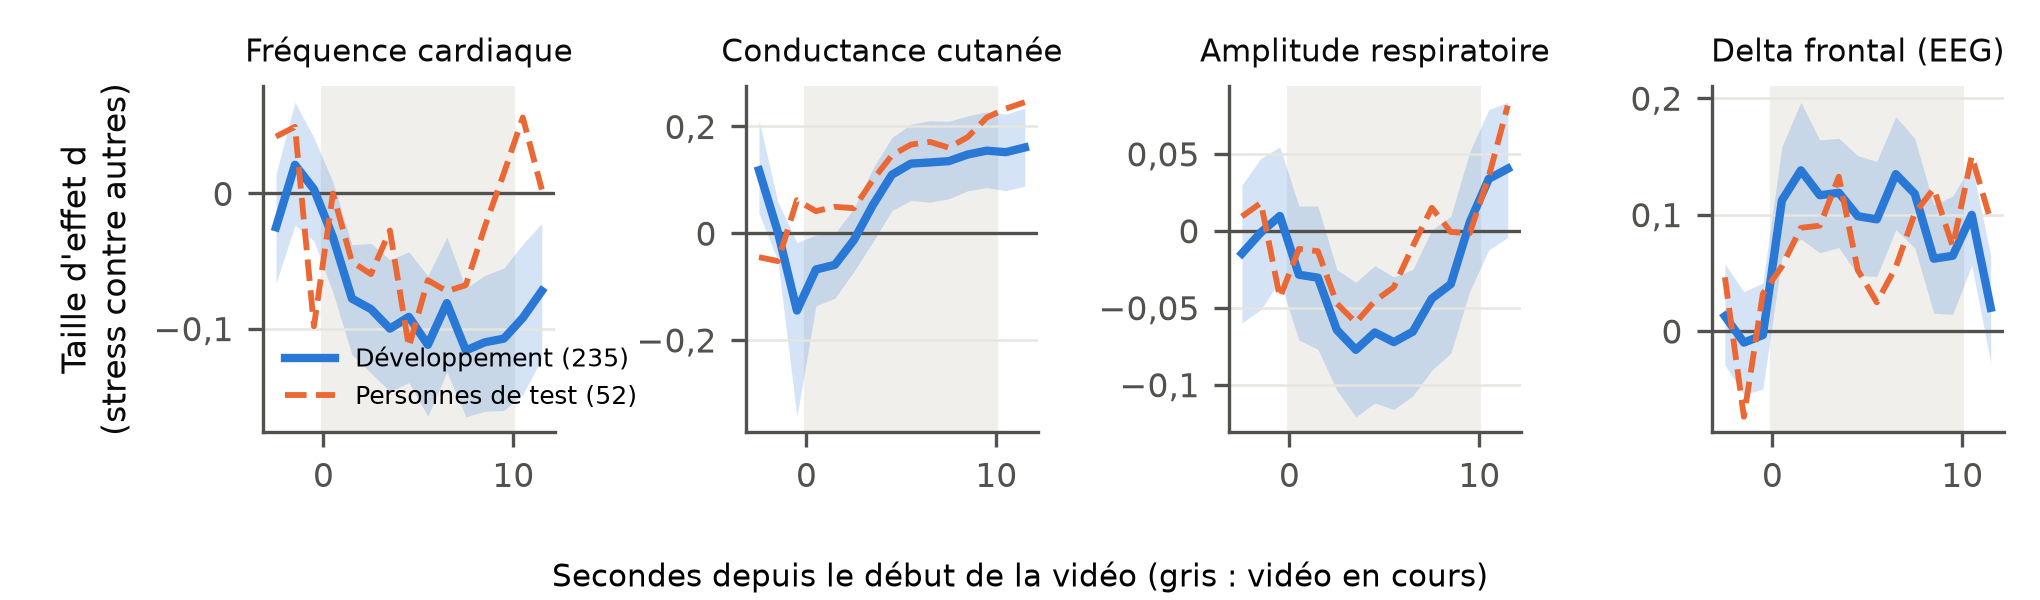
\includegraphics[width=0.95\linewidth]{curves_fr.png}
\caption{\textbf{Ordre d'apparition des réponses physiologiques seconde par seconde.} Taille d'effet intra-personne (stress contre autres essais) rapportée aux 3~s pré-stimulus. Bleu : 235 sujets de développement (bande IC 95\,\%). Orange tireté : réplication sur 52 sujets tenus à l'écart.}
\label{fig:curves}
\end{figure}

Après redressement automatique de la polarité inversée (96,6\,\% des essais), notre délinéation ECG couvre 94,7 à 98,7\,\% des 22\,974 essais avec des médianes cliniques normales : FC 76,3~bpm, RR 786,3~ms, pic PR 128,3~ms, PR clinique 134,9~ms, segment PR 39,9~ms, QRS 76,2~ms, QT 360,2~ms, QTc Bazett 402,7~ms, QTc Fridericia 386,9~ms, pic RT 250,2~ms et ratio T sur R de 0,53. Leur fiabilité entre les phases précoce et tardive de 5~s ($r = 0{,}45$ à $0{,}71$) est deux à trois fois supérieure à celle de la RMSSD ($0{,}22$).

Trois résultats électrophysiologiques se dégagent (figure~\ref{fig:ecg_eeg}A).
\begin{itemize}
\item L'intervalle RR s'allonge nettement pendant le stress ($+5{,}06$~ms, $d = +0{,}116$ [$+0{,}071 ; +0{,}163$]). L'effet est présent en phase précoce ($+0{,}092$), tardive ($+0{,}115$) et post-exposition ($+0{,}058$).
\item L'intervalle PR et le segment PR restent strictement nuls. Le pic PR varie de $-0{,}05$~ms ($d = -0{,}002$ [$-0{,}043 ; +0{,}036$]), le PR clinique de $+0{,}06$~ms ($+0{,}010$) et le segment PR pur de $-0{,}04$~ms ($-0{,}005$). Le contrôle sur $\Delta\mathrm{RR}$ ne révèle aucun effet caché ($-0{,}001$ à $-0{,}014$). La durée QRS ($+0{,}007$) et le ratio T sur R ($+0{,}025$) restent aussi nuls.
\item La baisse apparente du QTc est un artefact de formule. Les durées brutes RT ($+0{,}068$, $+0{,}22$~ms) et QT ($+0{,}047$, $+0{,}39$~ms) s'allongent à peine quand RR augmente, si bien que le QTc de Bazett baisse en apparence ($d = -0{,}092$ [$-0{,}140 ; -0{,}045$], $-1{,}00$~ms, et $-0{,}066$ pour Fridericia). Après contrôle sur $\Delta\mathrm{RR}$, tous ces effets disparaissent (QTc Bazett $-0{,}007$ [$-0{,}035 ; +0{,}020$], Fridericia $+0{,}014$, pic RT $+0{,}011$, QT $+0{,}034$). La repolarisation ventriculaire s'adapte plus lentement que 10~s, et la formule de Bazett sur-corrige la bradycardie rapide.
\end{itemize}

L'allongement de RR sans raccourcissement de PR (excluant un changement au-dessus de 0,3~ms) démontre que la réponse cardiaque sur 10~s est un freinage vagal sinusal, sans accélération adrénergique marquée au nœud atrio-ventriculaire.

\begin{figure}[t]
\centering
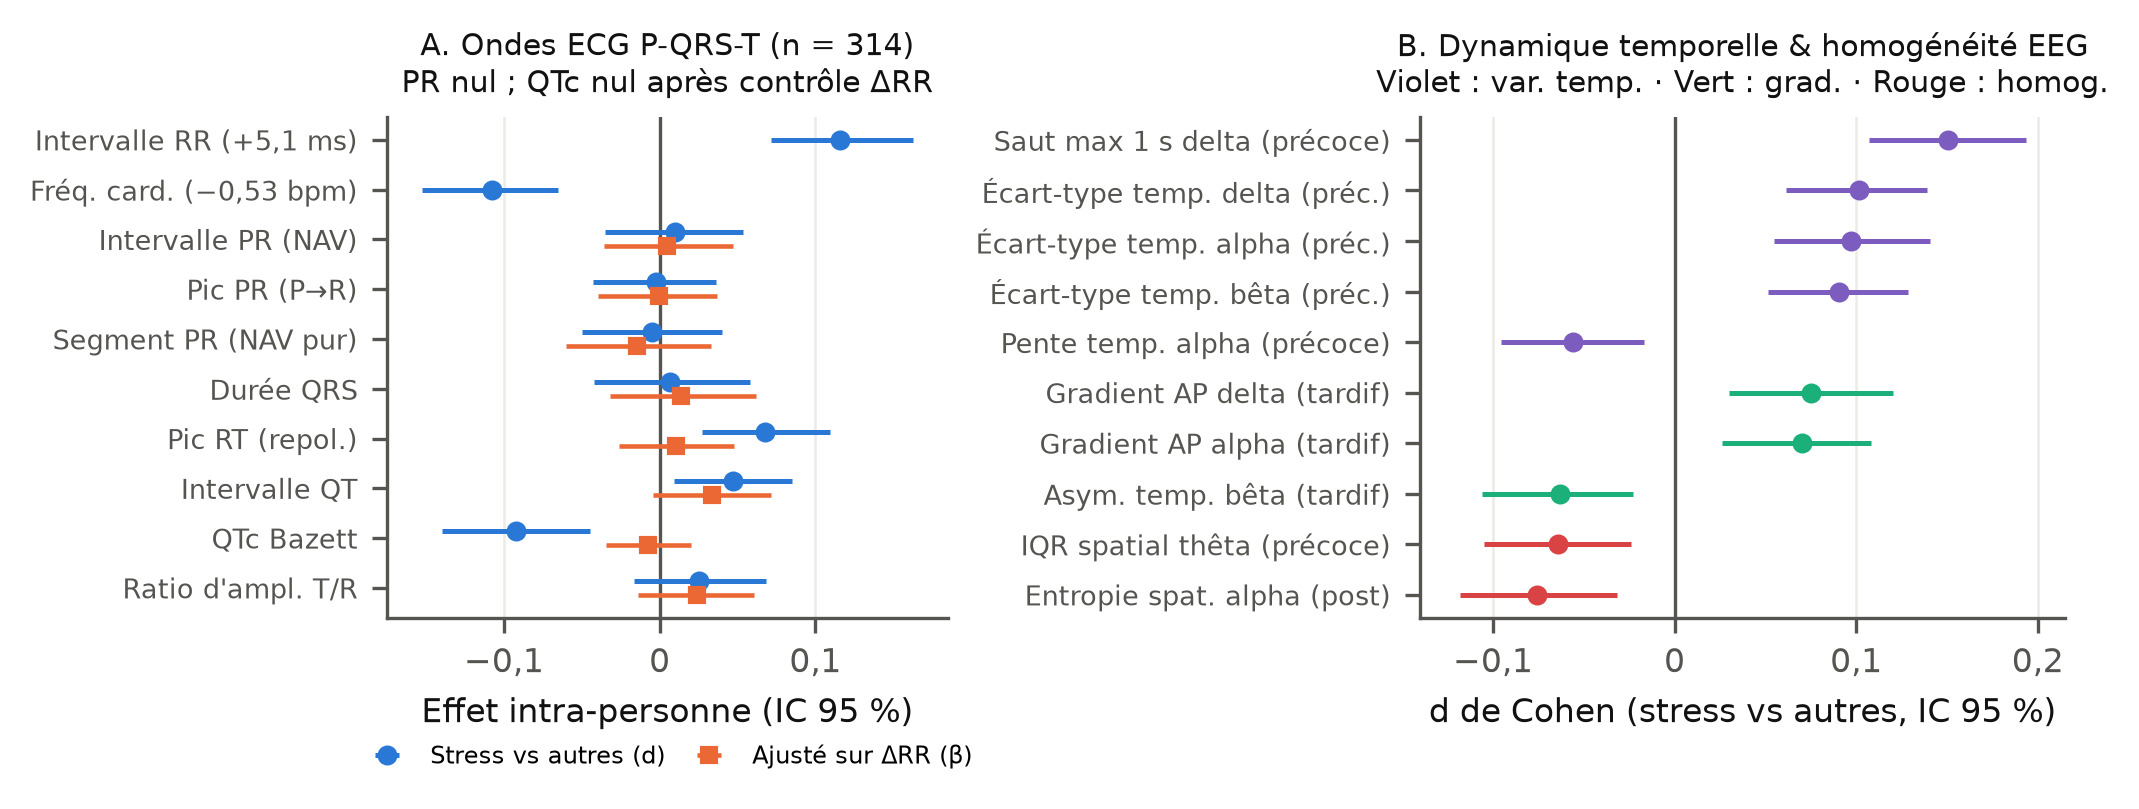
\includegraphics[width=\linewidth]{fig3_ecg_eeg_rich_fr.png}
\caption{\textbf{Morphologie ECG P-QRS-T et nouveaux descripteurs EEG.} \textbf{A.} Effets sur 10~s bruts (bleu) et ajustés sur $\Delta\mathrm{RR}$ (orange). RR s'allonge, PR et QRS sont nuls, et l'effet QTc disparaît après contrôle sur $\Delta\mathrm{RR}$. \textbf{B.} Effets des nouveaux descripteurs EEG : volatilité précoce (violet), gradients et asymétrie temporale (vert) et homogénéité spatiale biphasique (rouge).}
\label{fig:ecg_eeg}
\end{figure}

En EEG, les nouveaux descripteurs capturent en revanche des changements nets (figure~\ref{fig:ecg_eeg}B). En phase précoce ($0$ à $5$~s), l'écart-type temporel de la puissance 1~s augmente dans les cinq bandes ($\delta$ $+0{,}101$, $\alpha$ $+0{,}097$, $\theta$ $+0{,}096$, $\beta$ $+0{,}091$, $\gamma$ $+0{,}057$). Le plus grand saut de 1~s en delta atteint $d = +0{,}151$ [$+0{,}107 ; +0{,}193$]. Les pentes précoces sont négatives en alpha ($-0{,}056$) et en thêta ($-0{,}051$). Sur le plan spatial, la dispersion inter-canaux (\texttt{sp\_iqr}) diminue en phase précoce ($\theta$ $-0{,}064$, $\delta$ $-0{,}048$, $\gamma$ $-0{,}047$), indiquant une homogénéisation transitoire. Le motif s'inverse en phase tardive et post-exposition ($10$ à $12$~s), où l'entropie spatiale chute ($\alpha$ post $-0{,}076$ [$-0{,}118 ; -0{,}032$], $\theta$ post $-0{,}062$, $\delta$ post $-0{,}058$) pendant que l'écart-type inter-canaux monte ($+0{,}055$ à $+0{,}057$), montrant une focalisation spatiale persistante après la fin du clip. Enfin, le gradient antéro-postérieur bascule vers l'avant en phase tardive ($\delta$ $+0{,}075$, $\alpha$ $+0{,}070$, $\theta$ $+0{,}065$) et l'asymétrie temporale bêta dévie à gauche sur toute la durée ($-0{,}048$ précoce, $-0{,}063$ tardif, $-0{,}059$ post).

\subsection{Le prétraitement ICA ne masque pas de signal cerveau-cœur}

Sur les 287 participants évaluables (couverture 98,6\,\%, médiane 13 battements par vidéo, mêmes 62 électrodes et mêmes pics R), l'EEG brut sans ICA reproduit exactement le résultat de l'EEG nettoyé par ICA (figure~\ref{fig:hep_raw}).
\begin{itemize}
\item Sur \texttt{PREPROCESSED} (avec ICA, seuil 100\,$\mu$V), l'effet sur 250 à 600~ms vaut $d = +0{,}039$ [$-0{,}002 ; +0{,}078$], et $+0{,}039$ [$-0{,}002 ; +0{,}081$] après ajustement sur ECG et RR.
\item Sur \texttt{CURATED} (brut sans ICA, seuil 100\,$\mu$V), l'effet vaut $d = +0{,}038$ [$-0{,}001 ; +0{,}077$], et $+0{,}033$ [$-0{,}006 ; +0{,}073$] après ajustement sur ECG et RR. Au seuil élargi de 200\,$\mu$V, l'effet tombe à $+0{,}006$. Rapporté aux 3~s pré-stimulus, il vaut $-0{,}010$.
\item Le signal exact retiré par l'ICA (\texttt{CURATED} moins \texttt{PREPROCESSED}) ne montre aucune modulation par le stress ($d = +0{,}012$ [$-0{,}028 ; +0{,}053$]) et aucune corrélation avec le champ ECG ($r = -0{,}004$).
\item Un très faible effet positif apparaît seulement entre stress et relaxé, de façon identique avec ICA ($+0{,}072$ [$+0{,}014 ; +0{,}132$]) et sans ICA ($+0{,}076$ [$+0{,}021 ; +0{,}137$]).
\end{itemize}

L'ICA n'a donc pas détruit d'information cerveau-cœur. Avec environ 13 battements par essai de 10~s (contre 100 à 300 battements dans les études de conscience au repos \cite{park2014,candia2021}), la modulation du HEP par le stress aigu reste au plus très petite ($|d| < 0{,}08$).

\begin{figure}[t]
\centering
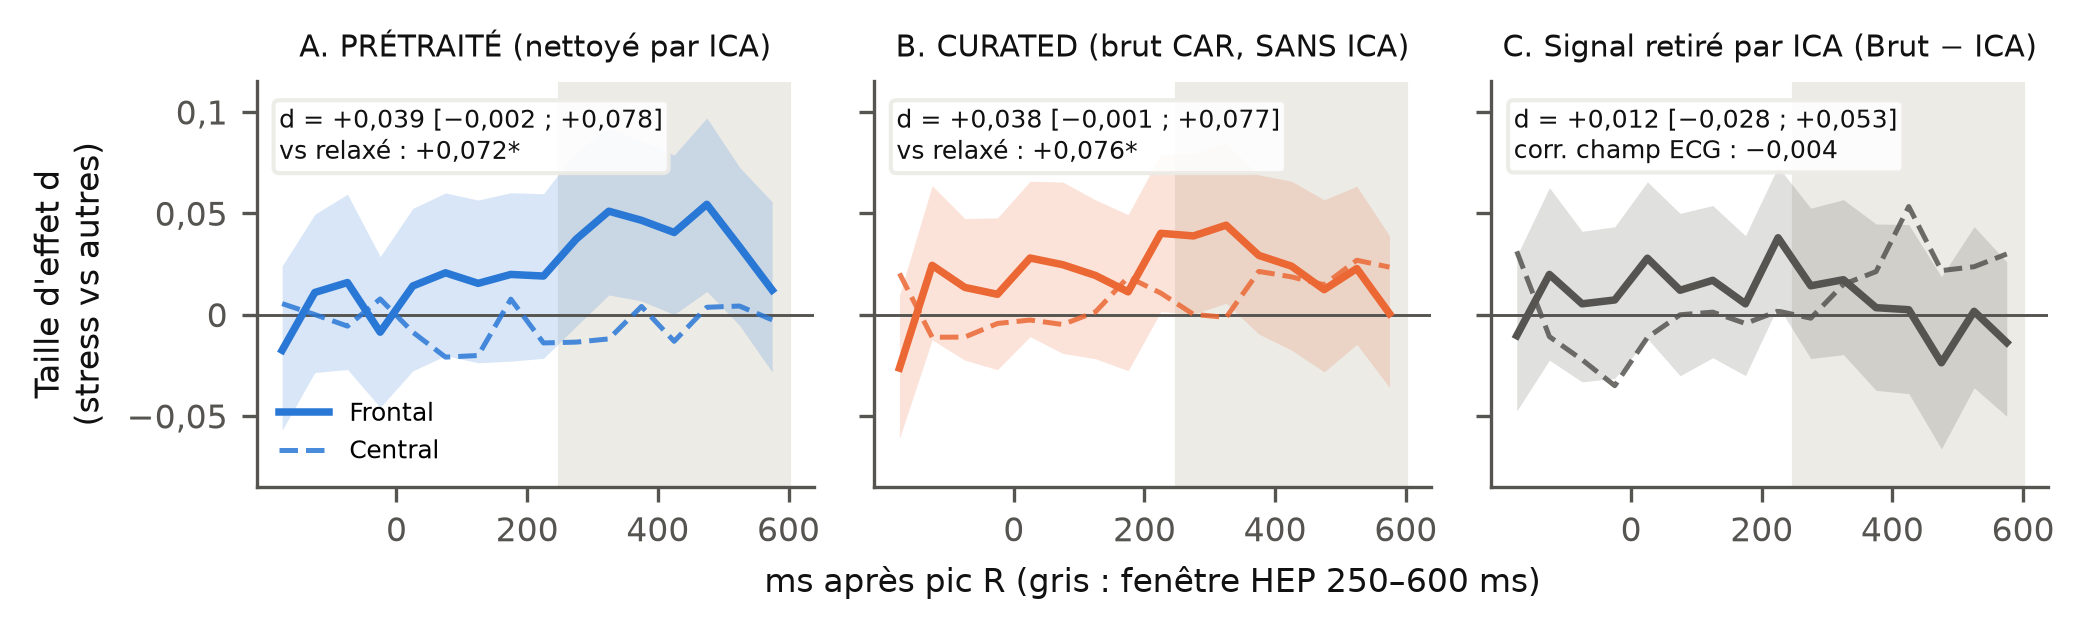
\includegraphics[width=\linewidth]{fig4_hep_raw_vs_ica_fr.png}
\caption{\textbf{Comparaison directe du potentiel évoqué cardiaque avec et sans ICA.} Effet stress contre autres essais chez 287 sujets sur les mêmes pics R et les 62 mêmes électrodes : \textbf{A.} \texttt{PREPROCESSED} (ICA). \textbf{B.} \texttt{CURATED} brut (sans ICA). \textbf{C.} Signal exact retiré par l'ICA.}
\label{fig:hep_raw}
\end{figure}

\subsection{À vidéo fixe, les spectateurs calmes ne décélèrent pas et seule l'alpha est automatique}

L'audit des 252 vidéos explique pourquoi notre étude 06 sous-estimait l'évaluation individuelle (figure~\ref{fig:fixed_video}C). Cent vingt-trois vidéos ont un taux de stress sous 10\,\%, 112 sont polarisantes (20 à 80\,\%) et 4 dépassent 80\,\%. Sur les vidéos consensuellement stressantes ($p_{v,-i} \ge 50\,\%$, $n = 5\,069$ essais), 63,9\,\% des spectateurs sont stressés et 33,6\,\% ($n = 1\,704$) sont dans la zone intermédiaire (par exemple valence négative mais arousal modéré). Seuls 2,5\,\% ($n = 124$, dont 63 très calmes) restent vraiment calmes. Comparer « stressé » contre « tout le reste » opposait donc 93\,\% du temps des stressés à des spectateurs déjà proches du seuil.

\begin{figure}[t]
\centering
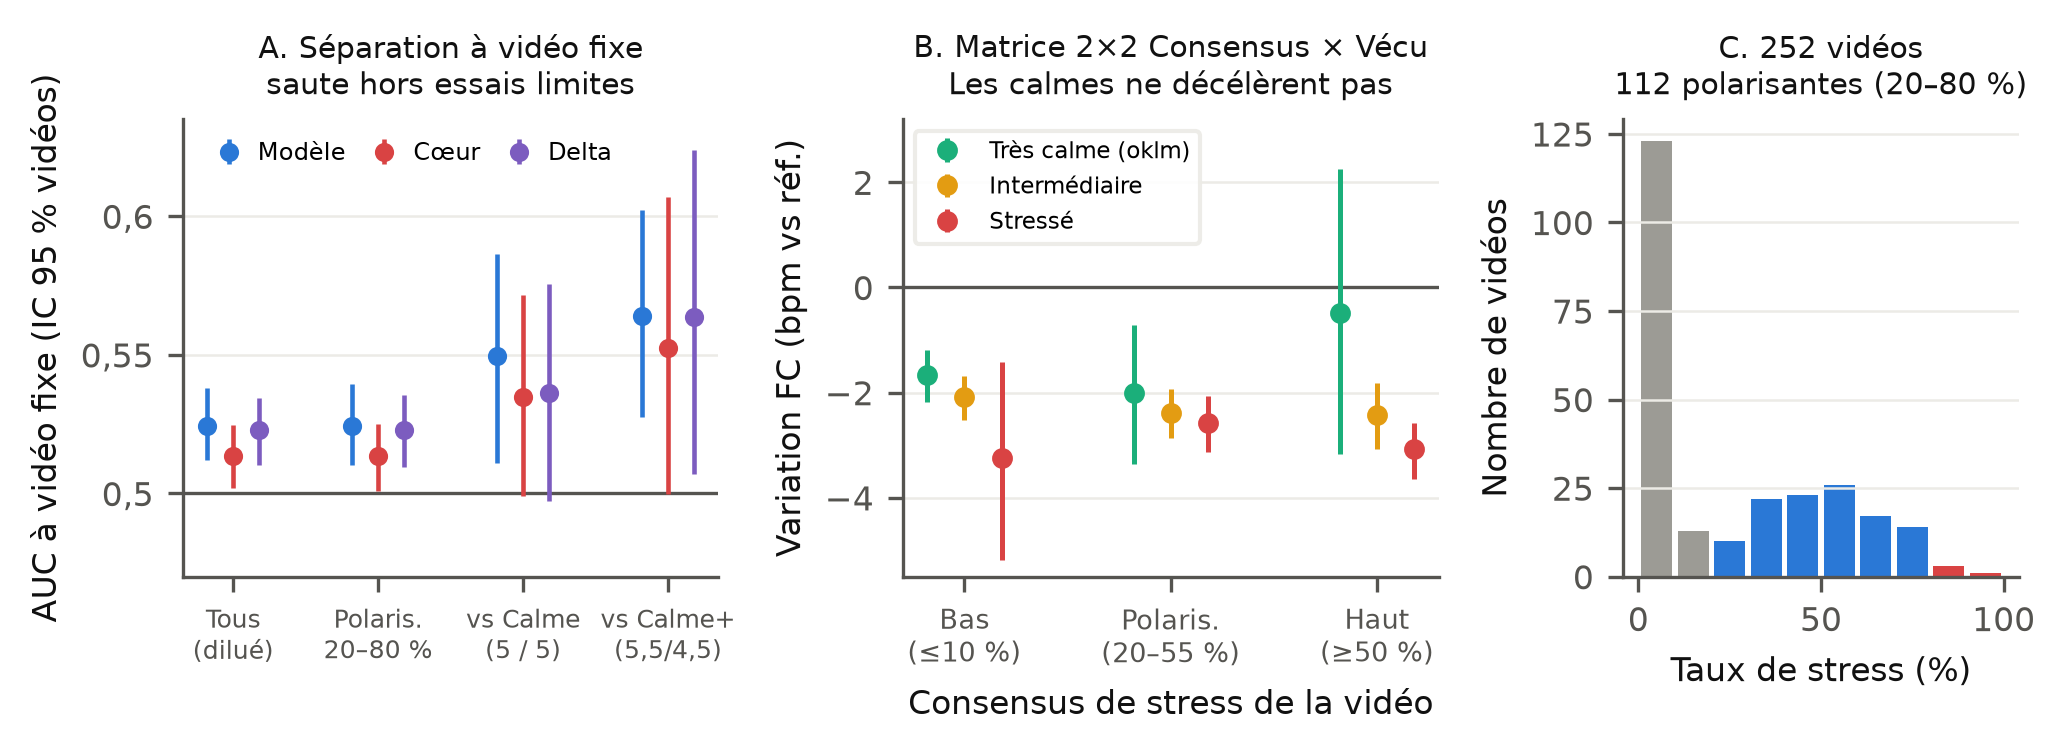
\includegraphics[width=\linewidth]{fig5_fixed_video_fr.png}
\caption{\textbf{Séparation à vidéo fixe et matrice $2 \times 2$ Consensus par état vécu.} \textbf{A.} L'AUC à vidéo fixe passe de 0,525 à 0,564 dès qu'on oppose les stressés aux spectateurs vraiment calmes devant la même vidéo. \textbf{B.} Variation de fréquence cardiaque par strate de consensus et d'état vécu. \textbf{C.} Répartition des taux de stress des 252 vidéos.}
\label{fig:fixed_video}
\end{figure}

Dès que l'on retire ces essais intermédiaires pour opposer stressés et spectateurs très calmes ($V \ge 5{,}5$ et $A \le 4{,}5$) devant la même vidéo (48 vidéos, 6\,403 paires), la séparation change nettement (figure~\ref{fig:fixed_video}A et B, tableau~\ref{tab:matrix2x2}).
\begin{itemize}
\item L'AUC à vidéo fixe passe de 0,525 [0,512 ; 0,538] à 0,564 [0,528 ; 0,602] pour le modèle multimodal, de 0,513 à 0,553 pour la fréquence cardiaque et de 0,523 à 0,564 pour le delta. L'effet intra-vidéo de la conductance cutanée double, de $+0{,}093$ à $+0{,}197$ ($+0{,}175$ [$+0{,}019 ; +0{,}320$] contre calme $5$ et $5$ sur 72 vidéos).
\item Dans la matrice $2 \times 2$ (tableau~\ref{tab:matrix2x2}), les spectateurs très calmes devant une vidéo consensuellement stressante ne montrent aucun ralentissement cardiaque ($-0{,}49$~bpm [$-3{,}16 ; +2{,}25$]) et aucune hausse de conductance cutanée ($+0{,}014\,\mu$S, exactement comme sur les vidéos neutres). Devant les mêmes clips, les spectateurs stressés affichent $-3{,}08$~bpm et $+0{,}041\,\mu$S. À l'inverse, quand une personne se sent stressée devant une vidéo consensuellement neutre ($n = 113$), son cœur ralentit de $-3{,}24$~bpm [$-5{,}19 ; -1{,}43$] et sa conductance cutanée monte de $+0{,}071\,\mu$S [$+0{,}022 ; +0{,}136$].
\item En comparaison appariée chez les mêmes personnes ($N = 26$ ayant été calmes sur certains clips stressants et stressées sur d'autres), l'effet évaluatif pur atteint $-2{,}97$~bpm [$-4{,}81 ; -1{,}10$] ($d = -0{,}41$ [$-0{,}65 ; -0{,}13$]) sur le cœur, $+0{,}033\,\mu$S ($d = +0{,}31$) sur la peau et $d = +0{,}45$ [$+0{,}00 ; +0{,}95$] sur le delta. En sens inverse, chez des sujets restés calmes devant des vidéos stressantes contre neutres ($N = 29$), seule la baisse d'alpha se déclenche automatiquement ($d = -0{,}33$ [$-0{,}56 ; -0{,}12$], et $-0{,}41$ chez les très calmes). Le cœur, la peau, la respiration et le delta ne bougent pas.
\end{itemize}

\begin{table}[t]
\centering\footnotesize
\setlength{\tabcolsep}{4.5pt}
\begin{tabular}{@{}llrrrrr@{}}
\toprule
Consensus vidéo ($p_{v,-i}$) & État du spectateur & Essais & Cœur (bpm) & Peau ($\mu$S) & Resp. & Delta ($\log_{10}$)\\
\midrule
Bas ($\le 10\,\%$) & Très calme ($V\ge 5{,}5, A\le 4{,}5$) & 4\,414 & $-1{,}67$ [$-2{,}17 ; -1{,}19$] & $+0{,}014$ & $-0{,}092$ & $-0{,}040$\\
 & Intermédiaire & 5\,831 & $-2{,}08$ [$-2{,}53 ; -1{,}68$] & $+0{,}025$ & $-0{,}156$ & $-0{,}049$\\
 & Stressé ($V\le 4, A\ge 6$) & 113 & $\mathbf{-3{,}24}$ [$-5{,}19 ; -1{,}43$] & $\mathbf{+0{,}071}$ & $-0{,}236$ & $-0{,}059$\\
\midrule
Polarisant (20 à 55\,\%) & Très calme & 167 & $-2{,}00$ [$-3{,}35 ; -0{,}71$] & $+0{,}021$ & $-0{,}197$ & $-0{,}094$\\
 & Intermédiaire & 3\,578 & $-2{,}39$ [$-2{,}85 ; -1{,}94$] & $+0{,}032$ & $-0{,}176$ & $-0{,}028$\\
 & Stressé & 2\,855 & $-2{,}58$ [$-3{,}14 ; -2{,}06$] & $\mathbf{+0{,}049}$ & $-0{,}188$ & $\mathbf{+0{,}009}$\\
\midrule
Haut ($\ge 50\,\%$) & Très calme & 63 & $\mathbf{-0{,}49}$ [$-3{,}16 ; +2{,}25$] & $\mathbf{+0{,}014}$ & $-0{,}111$ & $-0{,}073$\\
 & Intermédiaire & 1\,704 & $-2{,}43$ [$-3{,}08 ; -1{,}81$] & $+0{,}029$ & $-0{,}181$ & $-0{,}002$\\
 & Stressé & 3\,241 & $\mathbf{-3{,}08}$ [$-3{,}64 ; -2{,}57$] & $\mathbf{+0{,}041}$ & $-0{,}203$ & $\mathbf{+0{,}021}$\\
\bottomrule
\end{tabular}
\caption{Changements moyens par rapport aux 3~s pré-stimulus selon le consensus vidéo et l'état vécu (moyennes par participant avec IC bootstrap 95\,\%).}
\label{tab:matrix2x2}
\end{table}

Les courbes dose-réponse sur 8 tranches expliquent pourquoi la régression linéaire de l'étude 06 donnait une pente propre nulle alors qu'un effet évaluatif existe \cite{mauss2005,golland2014}. Sur la valence, la fréquence cardiaque suit un palier autour de 5. Elle est négative et plate entre 1 et 5 ($-0{,}42$ à $-0{,}20$~bpm), puis saute en positif dès $V \ge 5$ ($+0{,}52$ à $+0{,}54$~bpm). Sur l'arousal, la fréquence cardiaque décrit un U. Elle reste plate sous 5, atteint son creux maximal entre 6 et 7 ($-0{,}55$~bpm), puis remonte entre 7 et 9 ($+0{,}05$ à $+0{,}13$~bpm). La conductance cutanée et le delta restent plats jusqu'à 7 puis montent fortement entre 7 et 9 (peau $+0{,}014$ puis $+0{,}032\,\mu$S, delta $+0{,}016$ puis $+0{,}036$).

\subsection{La sensibilité individuelle suit le bêta et le gamma frontaux et le delta centro-pariétal}

La carte complète des 6 régions par 5 bandes montre où se situe la sensibilité propre à la valence négative (figure~\ref{fig:sens_models}A).
\begin{itemize}
\item Les pentes propres les plus fortes concernent le gamma frontal ($\beta_{\text{propre}} = -0{,}039$ [$-0{,}056 ; -0{,}022$]) et le bêta frontal ($-0{,}035$ [$-0{,}053 ; -0{,}017$]). Pour l'arousal propre, le gamma temporal gauche ressort aussi ($+0{,}030$ [$+0{,}013 ; +0{,}047$]). Sur les 62 électrodes, le bêta propre culmine en préfrontal bilatéral (Fp2 $-0{,}034$, Fp1 $-0{,}033$, AF7 $-0{,}029$, F4 $-0{,}028$, AF8 $-0{,}028$, F3 $-0{,}027$).
\item Le delta suit la valence propre dans les six régions, avec un maximum en central ($-0{,}037$ [$-0{,}053 ; -0{,}020$]) et sur les électrodes FC3 ($-0{,}041$), POz ($-0{,}041$), Pz ($-0{,}040$) et C3 ($-0{,}038$). Le proxy oculaire pré-ICA sur Fp1 et Fp2 corrèle avec le delta global ($\beta = +0{,}416$), mais son propre lien avec l'arousal vaut $+0{,}0004$ [$-0{,}017 ; +0{,}018$]. Après ajustement sur ce proxy, 93\,\% de l'effet propre du delta persiste ($+0{,}0286$ passe à $+0{,}0267$ [$+0{,}0102 ; +0{,}0423$]). L'effet delta n'est donc pas un artefact de clignement.
\item L'alpha, le thêta et l'asymétrie frontale (FAA) présentent des pentes propres nulles dans toutes les régions ($d = +0{,}021$ [$-0{,}023 ; +0{,}064$] pour la FAA alpha) \cite{vandervinne2017}.
\end{itemize}

Entre individus ($N = 314$, après ajustement sur la cohorte), les participants qui notent systématiquement les mêmes vidéos plus stressantes que leurs pairs ont une fréquence cardiaque de repos plus élevée ($r = +0{,}140$ [$+0{,}032 ; +0{,}244$]), un gamma pré-stimulus plus élevé sur tout le scalp (frontal $r = +0{,}165$ [$+0{,}061 ; +0{,}279$], Spearman $\rho = +0{,}185$), un thêta temporal pré-stimulus plus bas (temporal droit $r = -0{,}149$), et sont plus souvent des femmes ($r = +0{,}172$, $+0{,}226$ sur la valence négative \cite{bradley2001}). Ils ne présentent pas de réactivité phasique autonome plus forte ($r = -0{,}11$ sur la peau, non significatif). Ce profil basal rejoint les modèles d'hypervigilance anxieuse \cite{oathes2008}, avec la réserve d'une possible contribution micro-EMG résiduelle dans le gamma préfrontal et temporal.

\subsection{Les 4 phases enrichies surclassent les tranches de 1~s sur personnes et thèmes inédits}

Le benchmark des 12 configurations sur le nouveau découpage personnes par thèmes montre exactement quels choix améliorent la généralisation (figure~\ref{fig:sens_models}B et tableau~\ref{tab:seq_models}).
\begin{enumerate}
\item Passer des tranches de 1~s ($p = 340$) aux 4 phases physiologiques ($p = 114$) apporte le gain le plus simple. Avec trois fois moins de variables, l'AUC en développement passe de 0,546 à 0,560. Sur le test scellé strict (personnes et thèmes inédits), elle passe de 0,526 [0,481 ; 0,570] à 0,570 [0,519 ; 0,618]. Sur thèmes inédits, elle passe de 0,527 à 0,546.
\item Les ablations isolent les variables utiles. Partant des 4 phases avec transitions $\Delta(t\to t+1)$ (dév. 0,561, test strict 0,565), ajouter les ondes ECG P-QRS-T n'aide pas (dév. 0,559, test strict 0,562, thèmes inédits 0,540). Ajouter la volatilité temporelle EEG ($+30$ variables) donne le plus fort gain unitaire en développement (0,567, et AUC à vidéo fixe passant de 0,520 à 0,539) et porte le test strict à 0,580. Ajouter l'homogénéité spatiale EEG porte le test strict à 0,582 et donne la meilleure AUC à vidéo fixe sur thèmes inédits (0,542 [0,520 ; 0,562]).
\item Sur l'ensemble enrichi complet ($p = 448$), le modèle linéaire atteint 0,589 [0,540 ; 0,635] sur le test strict ($+0{,}063$ au-dessus des tranches de 1~s). La régression Ridge continue sur valence et arousal est le meilleur modèle global : 0,576 [0,561 ; 0,591] en développement, 0,586 [0,536 ; 0,633] sur le test strict (0,602 contre négatif calme), 0,558 [0,535 ; 0,581] sur thèmes inédits, et 0,607 [0,580 ; 0,633] sur sujets inédits (0,656 [0,623 ; 0,689] contre relaxé).
\item Exploiter la série de 1~s par convolutions 1D multi-échelles ($p = 620$) améliore nettement les mêmes données 1~s à plat (dév. 0,569 contre 0,546) et obtient la meilleure AUC à vidéo fixe en développement (0,541) et sur le test strict (0,527). En revanche, le GBDT perd en précision sur thèmes inédits (0,532) malgré un bon score sur thèmes vus (0,608), et le MLP sur les 1\,068 variables reste sous les modèles linéaires régularisés (dév. 0,552, thèmes inédits 0,531).
\end{enumerate}

\begin{figure}[t]
\centering
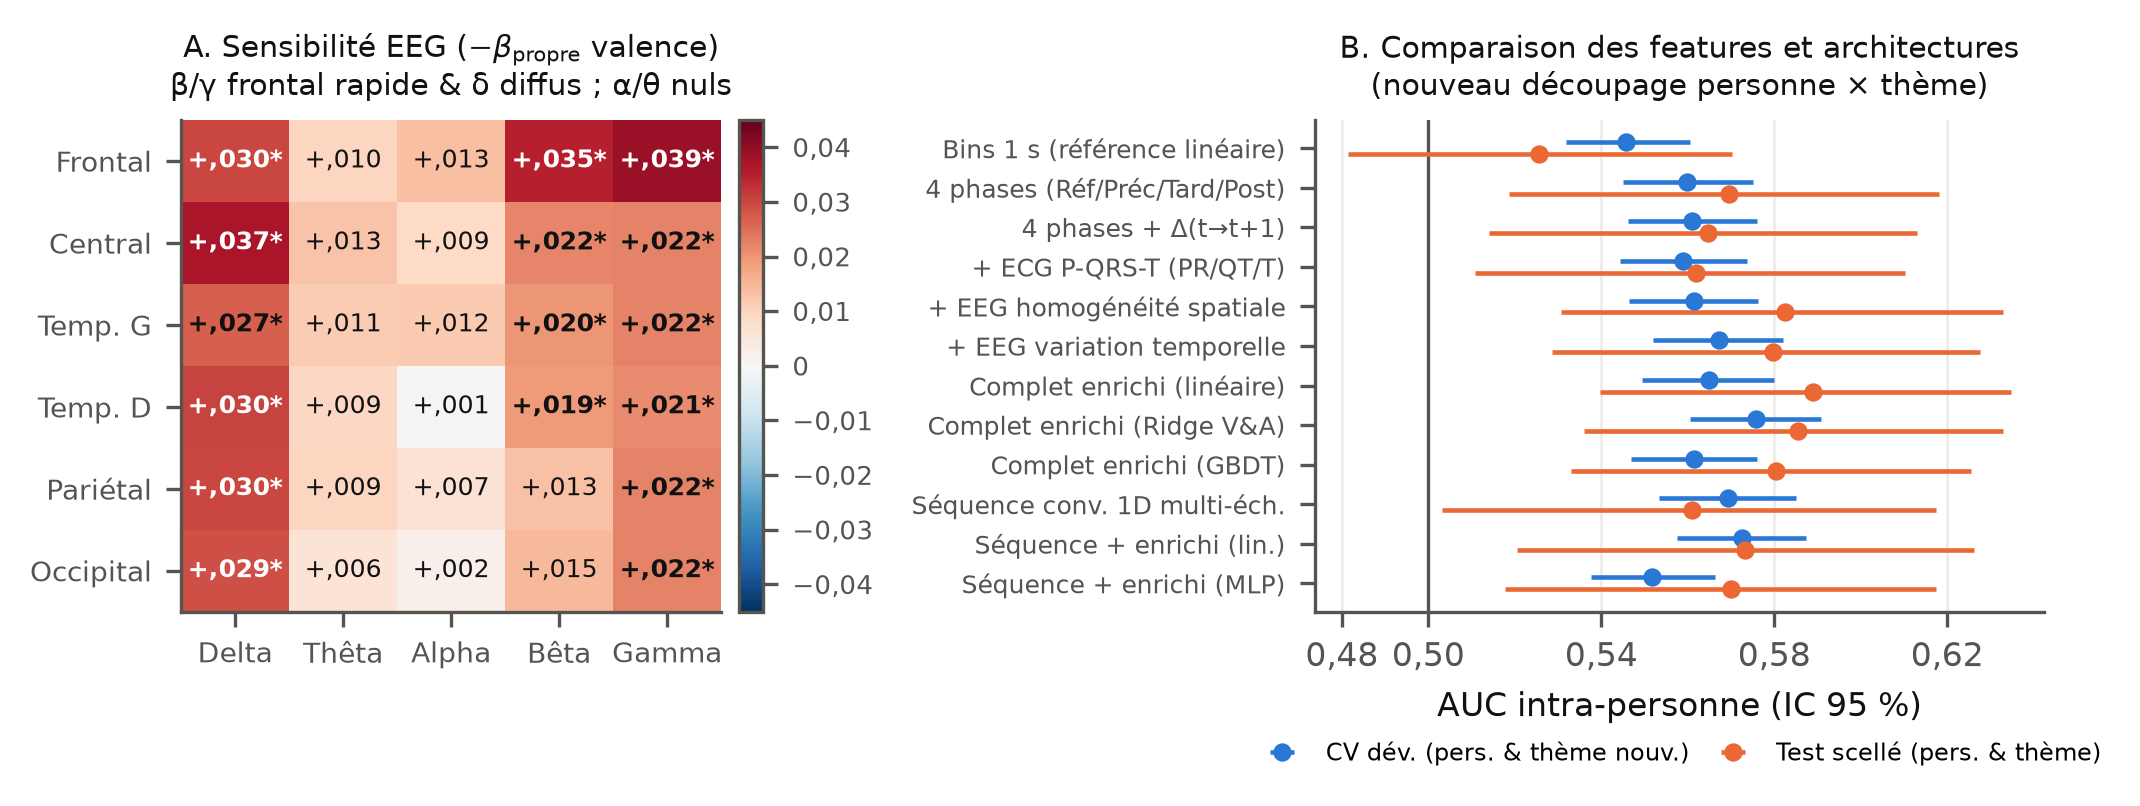
\includegraphics[width=\linewidth]{fig6_sensitivity_models_fr.png}
\caption{\textbf{Sensibilité EEG individuelle et comparaison des 12 configurations prédictives.} \textbf{A.} Matrice 6 régions par 5 bandes de $-\beta_{\text{propre}}$ sur la valence (* indique un IC 95\,\% excluant 0). \textbf{B.} AUC intra-personne sur le découpage \texttt{habs-revision-2026-11-23} en développement (bleu) et sur le test scellé personnes et thèmes nouveaux (orange).}
\label{fig:sens_models}
\end{figure}

\begin{table}[t]
\centering\footnotesize
\begin{tabular}{@{}lrrrrrrr@{}}
\toprule
Configuration & $p$ & Dév.\ WP & Dév.\ SV & Nouv.\ P\&T & Nouv.\ Pers. & Nouv.\ Th. & Contre relaxé (P)\\
\midrule
Tranches 1~s (référence lin.) & 340 & 0,546 & 0,519 & 0,526 & 0,600 & 0,527 & 0,632\\
4 phases (Réf, Préc, Tard, Post) & 114 & 0,560 & 0,524 & 0,570 & 0,599 & 0,546 & 0,632\\
4 phases et $\Delta(t\to t+1)$ & 190 & 0,561 & 0,520 & 0,565 & 0,605 & 0,548 & 0,650\\
\quad $+$ ECG P-QRS-T & 243 & 0,559 & 0,523 & 0,562 & 0,608 & 0,540 & 0,649\\
\quad $+$ EEG homogénéité spatiale & 365 & 0,562 & 0,521 & 0,582 & 0,600 & 0,555 & 0,640\\
\quad $+$ EEG variation temporelle & 220 & 0,567 & 0,539 & 0,580 & 0,599 & 0,547 & 0,640\\
Complet enrichi (linéaire) & 448 & 0,565 & 0,533 & \textbf{0,589} & 0,602 & 0,552 & 0,643\\
Complet enrichi (Ridge V et A) & 448 & \textbf{0,576} & 0,527 & 0,586 & 0,607 & \textbf{0,558} & \textbf{0,656}\\
Complet enrichi (GBDT) & 448 & 0,562 & 0,514 & 0,580 & \textbf{0,608} & 0,532 & 0,644\\
Séquence conv.\ 1D multi-échelles & 620 & 0,569 & \textbf{0,541} & 0,561 & 0,607 & 0,540 & 0,639\\
Séquence et enrichi (linéaire) & 1\,068 & 0,573 & 0,539 & 0,573 & 0,607 & 0,549 & 0,654\\
Séquence et enrichi (MLP) & 1\,068 & 0,552 & 0,527 & 0,570 & 0,608 & 0,531 & 0,648\\
\bottomrule
\end{tabular}
\caption{Performances des 12 configurations sur le découpage \texttt{habs-revision-2026-11-23}. WP : AUC intra-personne. SV : AUC à vidéo fixe pondérée. Nouv.\ P\&T : 65 sujets et 24 thèmes inédits. Nouv.\ Pers. : 65 sujets inédits. Nouv.\ Th. : 24 thèmes inédits.}
\label{tab:seq_models}
\end{table}

\section{Ce que ces résultats changent pour la neurophysiologie et le monitorage}

\begin{table}[t]
\centering\footnotesize
\begin{tabularx}{\linewidth}{@{}L{2.55cm} Y L{4.7cm}@{}}
\toprule
Question & Résultat vérifié & Chiffre clé\\
\midrule
Critère de stress & Validé sur émotions brutes. Durcir double la peau et le delta mais réduit la bradycardie. & 89,2\,\% rang 1 (97,2\,\% rangs 1 à 3). Optimum $3$ et $7$ (AUC 0,549).\\
Émotions et non sup. & Peur complète, dégoût vagal et delta, tristesse plate. Le clustering échoue. & Peur peau $+0{,}25$, cœur $-0{,}20$. $\mathrm{ARI} < 0{,}009$.\\
ECG P-QRS-T & RR s'allonge. PR reste nul. L'effet QTc disparaît après contrôle sur $\Delta\mathrm{RR}$. & RR $+5{,}1$~ms. PR $-0{,}05$~ms. QTc ajusté $-0{,}007$.\\
EEG enrichi & Forte volatilité précoce et organisation spatiale biphasique. & Saut delta $+0{,}151$. Entropie alpha post $-0{,}076$.\\
HEP brut et ICA & L'ICA ne retire aucun effet HEP caché. & Brut $+0{,}038$ contre ICA $+0{,}039$. Différence $+0{,}012$.\\
Vidéo fixe et $2\times 2$ & Retirer les essais limites révèle l'effet évaluatif. Seule l'alpha est automatique. & AUC vidéo fixe 0,564. Apparié cœur $-2{,}97$~bpm ($d = -0{,}41$).\\
Sensibilité EEG & Bêta et gamma frontaux, delta centro-pariétal (hors clignement), FC et gamma de repos. & Gamma frontal $-0{,}039$. Trait FC $+0{,}14$, gamma $+0{,}17$.\\
Modèles 4 phases & Les 4 phases enrichies et Ridge V et A battent les tranches 1~s. PR et MLP n'aident pas. & Test strict 0,526 à 0,589. Ridge dév. 0,576, relaxé 0,656.\\
\bottomrule
\end{tabularx}
\caption{Synthèse des résultats vérifiés sur 314 participants et 22\,974 essais.}
\label{tab:summary}
\end{table}

\subsection{Trois branches physiologiques distinctes pendant un stress aigu bref}

L'ensemble des mesures (tableau~\ref{tab:summary}) sépare trois réponses pendant une exposition aversive de 10~s :
\begin{enumerate}
\item Un réflexe attentionnel lié au stimulus. La baisse d'alpha pariéto-occipitale survient même quand le spectateur reste calme devant une vidéo stressante ($d = -0{,}33$ à $-0{,}41$) et ne suit pas l'évaluation propre.
\item Un freinage vagal déclenché par l'évaluation. Dès que la valence passe sous 5, la fréquence cardiaque baisse ($-2{,}4$ à $-3{,}1$~bpm dès 1~s) et la respiration devient plus superficielle (2~s), sans raccourcissement de PR ni variation de l'onde T. Cette bradycardie ne se produit pas chez un spectateur calme ($-0{,}49$~bpm).
\item Une alarme sympathique et corticale à seuil élevé. Au-dessus d'arousal 7, la conductance cutanée (4~s) et le delta centro-pariétal doublent. Le bêta et le gamma préfrontaux suivent la sensibilité individuelle, et la poussée sympathique cardiaque commence à contrer la bradycardie (courbe en U entre 8 et 9).
\end{enumerate}

\subsection{Règles pratiques pour les détecteurs et le monitorage clinique}

Quatre conséquences guident la conception de moniteurs non verbaux en neurofeedback, en recherche et chez les patients non communicants (douleur pédiatrique pré-verbale, \emph{locked-in syndrome}, coma, anesthésie générale) :
\begin{itemize}
\item Ne pas supposer une tachycardie linéaire. Un événement aversif bref ralentit d'abord le cœur (courbe en U avec l'arousal), alors qu'une douleur somatique intense ou un stress prolongé déclenche une tachycardie sympathique.
\item Éviter les métriques cardiaques instables sur 10~s. La RMSSD manque de fiabilité ($r_{\text{intra}} = 0{,}22$ à $0{,}43$), le QTc de Bazett sur-corrige quand RR varie vite, le segment PR ne montre pas de signal adrénergique mesurable et le HEP dispose de trop peu de battements ($\approx 13$).
\item Auditer les détecteurs avec trois indicateurs conjoints. Il faut rapporter l'AUC hors personne et hors stimulus, l'AUC à stimulus fixe entre états non adjacents (stressé contre calme) et la matrice $2 \times 2$ consensus par état vécu.
\item Ne pas fonder une décision clinique sur un seul extrait de 10~s. Malgré un gain net de $+0{,}030$ à $+0{,}063$ avec les 4 phases enrichies, l'AUC par essai plafonne entre 0,56 et 0,61 sur sujets et thèmes inédits (0,65 à 0,66 contre relaxé). Il faut donc agréger plusieurs épisodes et calibrer sur le niveau basal de chaque patient.
\end{itemize}

\subsection{Limites et reproductibilité}

Nos données proviennent de vidéos passives de 10~s chez des adultes sains. Un stress actif ou une douleur aiguë en pédiatrie recrutent plus fortement la voie adrénergique (tachycardie et possible raccourcissement PR au-delà de 10 à 30~s). La dérivation ECG unique empêche toute analyse vectorielle multi-dérivations. La cellule extrême des spectateurs très calmes devant des vidéos très stressantes reste petite ($n = 63$, 26 sujets appariés). Notre contrôle oculaire pré-ICA écarte le clignement pour le delta centro-pariétal, mais un micro-EMG crânien résiduel peut encore contribuer au bêta et au gamma préfrontaux et temporaux. Enfin, l'absence de notations répétées d'une même vidéo par une même personne empêche de mesurer directement la fiabilité test-retest des notes.

Le code d'extraction (\texttt{decoding/\allowbreak rich\_extract.py}), le code d'analyse (\texttt{decoding/\allowbreak revision.py}), le protocole figé (\texttt{journal/\allowbreak 07\_comprehensive\_revision.md}), les agrégats JSON et le script des figures (\texttt{docs/\allowbreak research/\allowbreak revision/\allowbreak make\_figures.py}) sont versionnés dans le dépôt. Aucune donnée individuelle ne quitte les serveurs HABS.

\begin{otherlanguage*}{english}
\begin{thebibliography}{99}\footnotesize\setlength{\itemsep}{1.2pt}
\bibitem{giannakakis2015} G. Giannakakis, D. Grigoriadis, M. Tsiknakis. Detection of stress/anxiety state from EEG features during video watching. IEEE EMBC 2015, 6034--6037.
\bibitem{gerster2026} M. Gerster et al. Stimulus identity rather than emotion drives EEG classification on the FACED dataset. bioRxiv 2026, doi:10.64898/2026.06.12.731889.
\bibitem{bradley2001} M. M. Bradley, M. Codispoti, D. Sabatinelli, P. J. Lang. Emotion and motivation II: sex differences in picture processing. Emotion 1 (2001) 300--319.
\bibitem{bradley2009} M. M. Bradley. Natural selective attention: orienting and emotion. Psychophysiology 46 (2009) 1--11.
\bibitem{benedek2010} M. Benedek, C. Kaernbach. A continuous measure of phasic electrodermal activity. J. Neurosci. Methods 190 (2010) 80--91.
\bibitem{lang1993} P. J. Lang, M. K. Greenwald, M. M. Bradley, A. O. Hamm. Looking at pictures: affective, facial, visceral, and behavioral reactions. Psychophysiology 30 (1993) 261--273.
\bibitem{palomba2000} D. Palomba, M. Sarlo, A. Angrilli, A. Mini, L. Stegagno. Cardiac responses associated with affective processing of unpleasant film stimuli. Int. J. Psychophysiol. 36 (2000) 45--57.
\bibitem{hagenaars2014} M. A. Hagenaars, K. Roelofs, J. F. Stins. Human freezing in response to affective films. Anxiety, Stress, \& Coping 27 (2014) 27--37.
\bibitem{schubring2019} D. Schubring, H. T. Schupp. Affective picture processing: alpha- and lower beta-band desynchronization reflects emotional arousal. Psychophysiology 56 (2019) e13386.
\bibitem{siegel2018} E. H. Siegel et al. Emotion fingerprints or emotion populations? A meta-analytic investigation of autonomic features of emotion categories. Psychol. Bull. 144 (2018) 343--393.
\bibitem{mauss2005} I. B. Mauss et al. The tie that binds? Coherence among emotion experience, behavior, and physiology. Emotion 5 (2005) 175--190.
\bibitem{golland2014} Y. Golland, K. Keissar, N. Levit-Binnun. Studying the dynamics of autonomic activity during emotional experience. Psychophysiology 51 (2014) 1101--1111.
\bibitem{park2014} H.-D. Park, S. Correia, A. Ducorps, C. Tallon-Baudry. Spontaneous fluctuations in neural responses to heartbeats predict visual detection. Nat. Neurosci. 17 (2014) 612--618.
\bibitem{candia2021} D. Candia-Rivera et al. Neural responses to heartbeats detect residual signs of consciousness during resting state in postcomatose patients. J. Neurosci. 41 (2021) 5251--5262.
\bibitem{parkblanke2019} H.-D. Park, O. Blanke. Heartbeat-evoked cortical responses: underlying mechanisms, functional roles, and methodological considerations. NeuroImage 197 (2019) 502--511.
\bibitem{munoz2015} M. L. Munoz et al. Validity of (ultra-)short recordings for heart rate variability measurements. PLoS ONE 10 (2015) e0138921.
\bibitem{vandervinne2017} N. van der Vinne et al. Frontal alpha asymmetry as a diagnostic marker in depression: fact or fiction? A meta-analysis. NeuroImage: Clinical 16 (2017) 79--87.
\bibitem{oathes2008} D. J. Oathes, W. J. Ray, A. S. Yamasaki, T. D. Borkovec, L. G. Castonguay, M. G. Newman, J. Nitschke. Worry, generalized anxiety disorder, and emotion: evidence from the EEG gamma band. Biol. Psychol. 79 (2008) 165--170.
\bibitem{varoquaux2018} G. Varoquaux. Cross-validation failure: small sample sizes lead to large error bars. NeuroImage 180 (2018) 68--77.
\end{thebibliography}
\end{otherlanguage*}

\end{document}
